\documentclass[a4paper]{ctexart}
\usepackage{amsmath, amsthm, amssymb, graphicx}
\usepackage{setspace}
%\usepackage[bookmarks=true, colorlinks, citecolor=blue, linkcolor=black]{hyperref}

% 导言区

\title{C++程序设计大作业报告}
\date{\today}
\pagestyle{plain}

\begin{document}
        \thispagestyle{empty}
    	\begin{figure}[t]
		\parbox[b]{2cm}{
			}
		\parbox[b]{9cm}{
			\begin{center}

				%\small \textbf{SOUTHEAST\quad UNIVERSITY} 
			\end{center}
			}
	\end{figure}

	\begin{center}
		\quad \\
		\quad \\
		\heiti \fontsize{25}{17} 程\quad 序\quad 设\quad 计\quad 大\quad 作\quad 业\quad 报\quad 告
		\vskip 2.5cm
		\heiti \zihao{2} 	
	\end{center}
	\vskip 2.5cm

	\begin{quotation}
		\songti \fontsize{15}{15}
		\doublespacing
		\par\setlength\parindent{12em}
		\quad 

        作业名称:\underline{\quad 城市天际线\quad}


		学\hspace{0.61cm} 院:\underline{\quad 材料学院\qquad}
        
        班\hspace{0.61cm} 级:\underline{\qquad 04102301\quad}

		学生姓名:\underline{\qquad 白昊明\qquad }

		学\hspace{0.61cm} 号:\underline{\quad 2023301350\quad}

		\vskip 2cm
        \centering
		西北工业大学
		\vskip 0cm
		\centering
		2023年12月2日
	\end{quotation}
    \textbf{}
    \begin{abstract}
        本次大作业选择的是上的ACM模拟试题,题目的主要要求是根据给出的矩形建筑物的上沿,输出城市的天际线的顶点向量。
		本次作业使用了C++风格的文件流操作,代码更加简洁易懂,并且融入了面向对象编程的思想。
		本次作业基本完成既定目标,实现了预期功能,但是对数据执行了三次循环,执行效率尚有待提高。
		本次作业思路清晰明确,运用了高级工具,运用了C++特有的功能和特性。
    \end{abstract}
    \newpage

	\tableofcontents
	\newpage
	\section{摘要}
	\subsection{设计题目}
	英文名称:Skyline

	中文名称:城市天际线
	\subsection{设计内容}
	\paragraph{英文原文}~

	ACM: Draw the skyline of a city according to the data given by the input file.
	
	With the advent of high speed graphics workstations, CAD (computer-aided design) and other areas (CAM, VLSI design) have made increasingly effective use of computers. One of the problems with drawing images is the elimination of hidden lines — lines obscured by other parts of a drawing.

	You are to design a program to assist an architect in drawing the skyline of a city given the locations of the buildings in the city. To make the problem tractable, all buildings are rectangular in shape and they share a common bottom (the city they are built in is very flat). The city is also viewed as two-dimensional. A building is specified by an ordered triple ($L_i$, $H_i$, $R_i$) where $L_i$ and $R_i$ are the left and right coordinates, respectively, of building $i$ (0 $\textless$  $L_i$ $\textless$  $R_i$) and $H_i$ is the height of the building. In the diagram below buildings are shown on the left with triples.

	(1,11,5),(2,6,7),(3,13,9),(12,7,16),(14,3,25),(19,18,22),(23,13,29),(24,4,28)

	The skyline, shown on the right, is represented by the sequence:

	(1,11,3,13,9,0,12,7,16,3,19,18,22,3,23,13,29,0)

	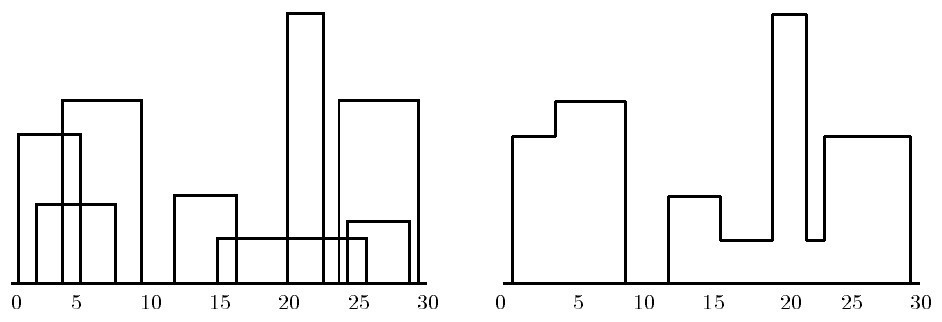
\includegraphics[width=10.465cm,height=3.577cm]{effect.jpg}

	\textbf{Input}

	The input is a sequence of building triples. All coordinates of buildings are integers less than 10,000 and there will be at least one and at most 5,000 buildings in the input file. Each building triple is on a line by itself in the input file. All integers in a triple are separated by one or more spaces. The triples will be sorted by Li, the left x-coordinate of the building, so the building with the smallest left x-coordinate is first in the input file.

	\textbf{Output}

	The output should consist of the vector that describes the skyline as shown in the example above.
	
	In the skyline vector ($v_1$,$v_2$,$v_3$,...,$v_n-2$,$v_n-1$,$v_n$), the $v_i$ such that $i$ is an even number represent a horizontal line (height). The vi such that $i$ is an odd number represent a vertical line (x-coordinate). The skyline vector should represent the "path" taken, for example, by a bug starting at the minimum x-coordinate and traveling horizontally and vertically over all the lines that define the skyline. Thus the last entry in all skyline vectors will be a '0'.
	
	\textbf{Sample Input}

	1 11 5

	2 6 7

	3 13 9

	12 7 16

	14 3 25

	19 18 22

	23 13 29

	24 4 28

	\textbf{Sample Output}

	1 11 3 13 9 0 12 7 16 3 19 18 22 3 23 13 29 0



	\paragraph{中文翻译}~

	ACM模拟试题:根据输入文件中给出的数据描绘一个城市的天际线。

	随着高速计算机的流行,CAD(计算机辅助设计软件)和其他的领域(CAM,VLSI设计等)已经越发高效地使用着计算机。图形绘制中,怎样消去隐藏的直线——即那些被绘制图形的其他部分遮挡的直线——是一个问题。

	你将要设计一个程序以辅助建筑师通过输入城市中建筑的位置描绘城市的天际线。为了简化这个问题,我们假设所有的建筑都是矩形并且它们的底部高度相同(这个城市的地面非常的平坦)。同样地,城市也被看作一个二维的平面(正垂面)。在题目中,每座建筑都用一组三元数据表示 ($L_i$, $H_i$, $R_i$) 。其中,$L_i$和$R_i$分别表示建筑 $i$ 两侧边的所在位置的横坐标。下方示意图中的建筑可以用如下的一行三元数据表示:

	(1,11,5),(2,6,7),(3,13,9),(12,7,16),(14,3,25),(19,18,22),(23,13,29),(24,4,28)

	而图中右半部分展示的天际线则可以用如下的一组数列表示:

	(1,11,3,13,9,0,12,7,16,3,19,18,22,3,23,13,29,0)
	
	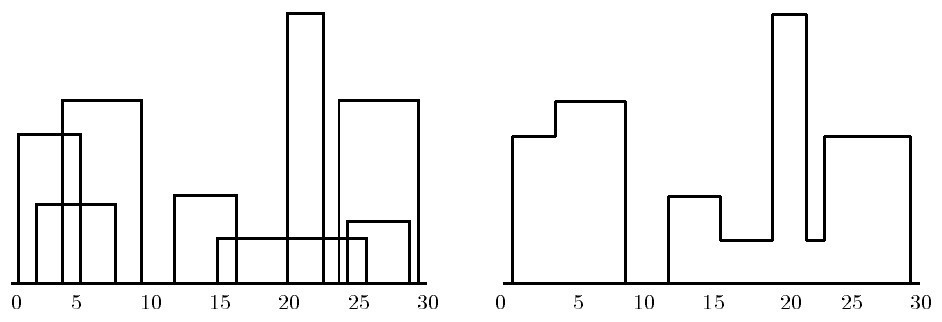
\includegraphics[width=10.465cm,height=3.577cm]{effect.jpg}

	\textbf{输入}
	
	输入的是是一个表示建筑的三元数据的序列。所有的坐标值都是小于10000的整数并且输入文件中建筑的数量不会超过5000座。每一座建筑的坐标数据和它在输入文件中独立成行。同一组数据的两个整数之间用一个或者几个空格分隔。数据已经根据$L_i$从小到大排序,所以有着最小的横坐标的建筑将会第一个出现在输入文件中



	\subsection{开发工具}
	\subsection{应用平台}
	\section{详细设计}
	\subsection{程序结构}
	\subsection{主要功能}
	\subsection{函数实现}
	\subsection{开发日志}
	\section{程序调试及运行}
	\subsection{程序运行结果}
	\subsection{程序使用说明}
	\subsection{程序开发总结}
	\section{附件(源程序)}

\end{document}